\documentclass[border={-4pt -6pt -4pt -4pt}]{standalone}

\usepackage{hyperref}
\usepackage{tikz}

\usetikzlibrary{decorations.pathreplacing,
  arrows,
  calc,
  decorations.pathmorphing,
  decorations.pathreplacing,
  decorations.markings,
  positioning,
  shapes,
  3d
}

\ifpdf
% Ensure reproducible output
\pdfinfoomitdate=1
\pdfsuppressptexinfo=-1
\pdftrailerid{}
\hypersetup{
  pdfcreator={},
  pdfproducer={}
}
\fi

\begin{document}
\begin{tikzpicture}
  \node at (0.0, 0) {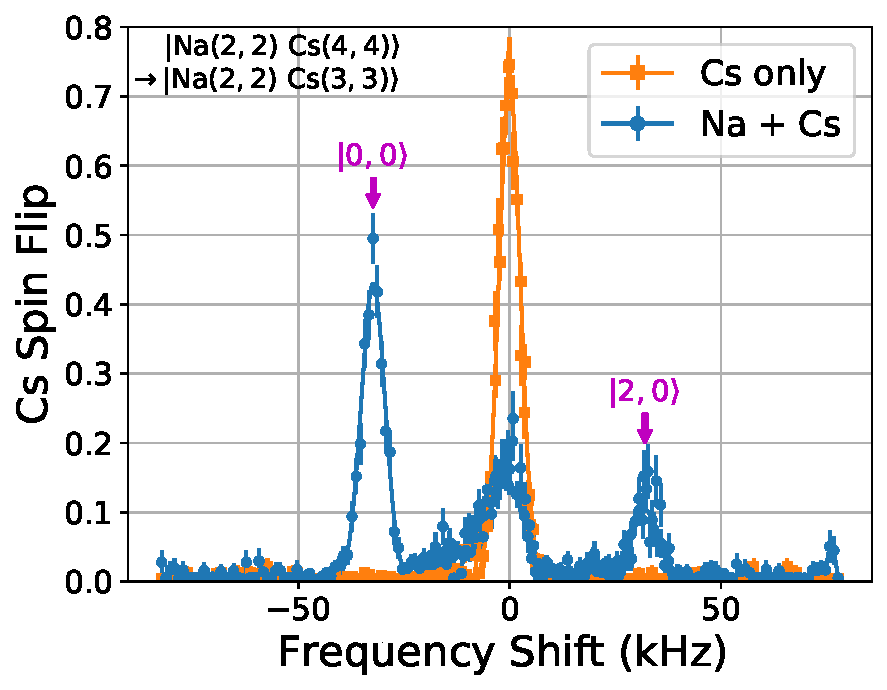
\includegraphics[height=4.5cm]{interaction_shift_spectrum_42_32.pdf}};
  \node at (6.1, -0.05) {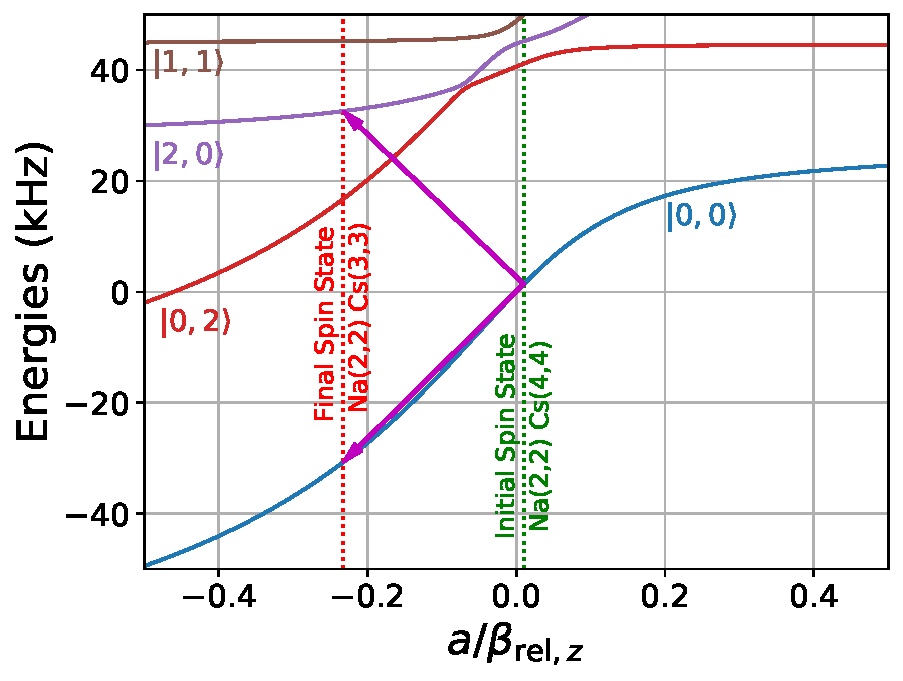
\includegraphics[height=4.5cm]{interaction_shift_energies_42_32.pdf}};
  \node at (-2.65, 1.85) {\scriptsize (\textbf{A})};
  \node at (3.40, 1.85) {\scriptsize (\textbf{B})};
  \begin{scope}[shift={(0, -4.6)}]
    \node at (0.0, 0) {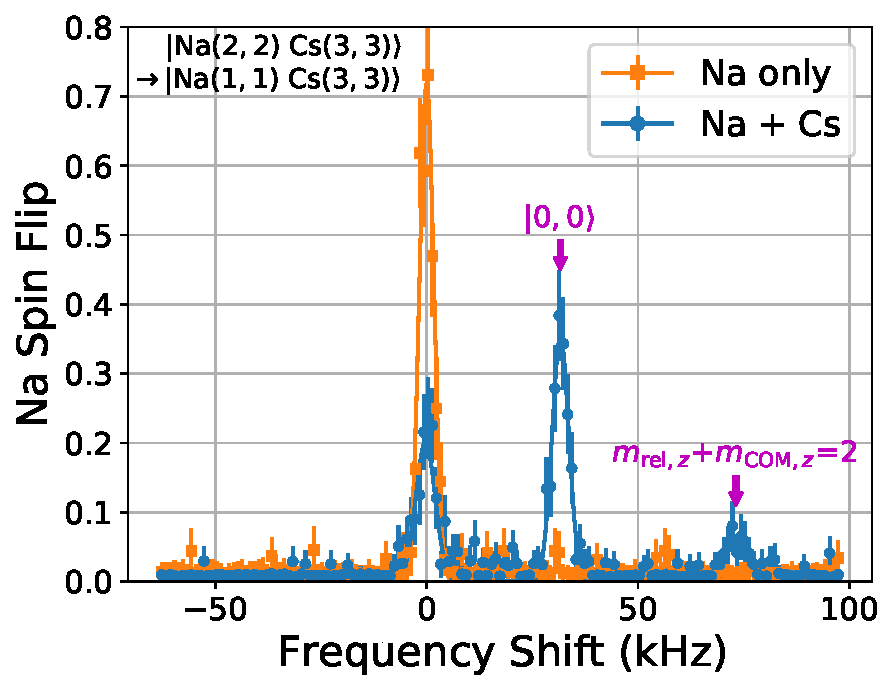
\includegraphics[height=4.5cm]{interaction_shift_spectrum_32_31.pdf}};
    \node at (6.1, -0.05) {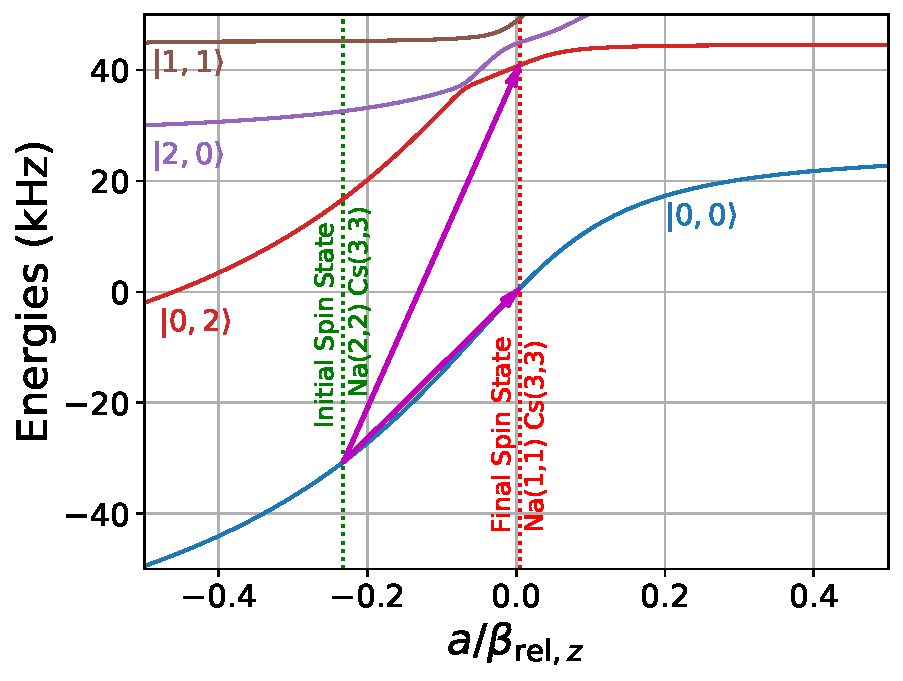
\includegraphics[height=4.5cm]{interaction_shift_energies_32_31.pdf}};
    \node at (-2.65, 1.85) {\scriptsize (\textbf{C})};
    \node at (3.40, 1.85) {\scriptsize (\textbf{D})};
  \end{scope}
\end{tikzpicture}
\end{document}
